\documentclass[conference]{acmsiggraph}

\usepackage{cleveref}

\title{The Title of Your Paper Goes Here}

%%%%%%%%%%%%%%%%%%%%%%%%%%%%
% authors
%%%%%%%%%%%%%%%%%%%%%%%%%%%%
\author{
	Felix Manke\thanks{e-mail: felix.manke@campus.lmu.de}\\LMU Munich
	\and
	Tibor Goldschwendt\thanks{e-mail: goldschwendt@cip.ifi.lmu.de}\\LMU Munich
	\and
	Oleg Maltsev\thanks{e-mail: ga49bof@mytum.de}\\TU Munich
}
	
\pdfauthor{Felix Manke, Tibor Goldschwendt}

\keywords{radiosity, global illumination, constant time}

\begin{document}

%% \teaser{
%%   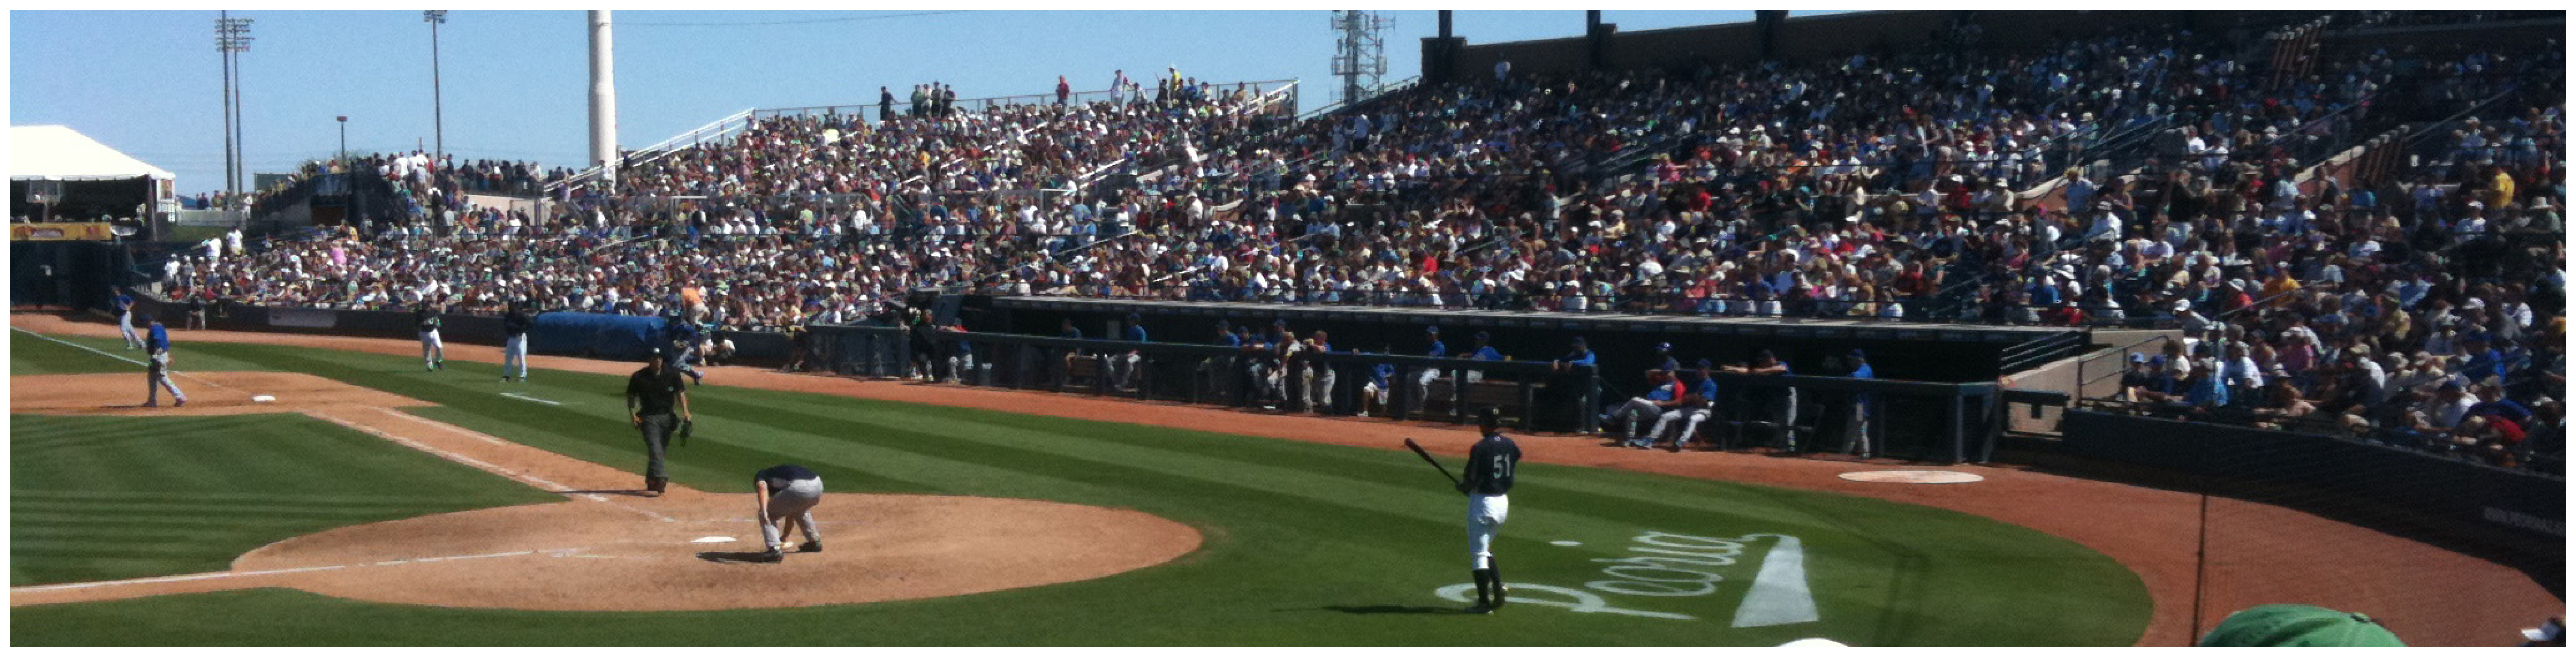
\includegraphics[height=1.5in]{images/sampleteaser}
%%   \caption{Spring Training 2009, Peoria, AZ.}
%% }

\maketitle


%%%%%%%%%%%%
% ABSTRACT %
%%%%%%%%%%%%

\begin{abstract}

\end{abstract}

\copyrightspace




%%%%%%%%%%%%%%%%
% INTRODUCTION %
%%%%%%%%%%%%%%%%

\section{Introduction}

\begin{itemize}
\item motivation
\item{
	general description of the project
	\begin{itemize}
	\item what is it\\
	 ($\rightarrow$ introductory text from wiki... separation of senses, visual, tactile, ...)
	\item dark room side (explanation of dark room: what happens there, what does the user do. Not too technical\\
	 $\Rightarrow$ only the concept)
	\item communication
	(point out, that data gets transmitted over to the cave so that there is a spatial separation as well)
	\item CAVE-side\\
	(how does the interaction in the cave look like? what happens there? How does the room-user affect the cave-environment and vice versa...)
	\end{itemize}
}
\item entire team\\
	  (describe, who worked on the project... what about a complete list of all names in the appendix maybe, like credits in a movie or video game?)
\item aspects: arts vs. technology\\
		(combination of both worlds, merging the best aspects, creating an immersive installation)
\item how we find the concept\\
		(description of the development process $\Rightarrow$ time (October till March... still ongoing to prepare it for future exhibitions...), presence meetings in Munich and Linz aka. Workshops, several Skype-Meetings, different approaches and ideas (interactive table, visualising time, ... , finally: separation of senses) 
\item purpose of this paper
\end{itemize}

\section{Implementation}




%%%%%%%%%%%%%%%%%%%%%%%%%%%%
% APPLICATION ARCHITECTURE %
%%%%%%%%%%%%%%%%%%%%%%%%%%%%

\subsection{General Application Architecture}
\textit{Graphic / diagram} to visualize the overall system architecture (room-components, network, cave-components)
\begin{itemize}
\item brief description of components
\end{itemize}




%%%%%%%%%%%
% NETWORK %
%%%%%%%%%%%

\subsection{Network}
\begin{itemize}
\item introduction
\item{
	used technologies
	\begin{itemize}
	\item Liblo + OSC
	\end{itemize}
}
\item evolution over time
\item{
	detailed description
	\begin{itemize}
	\item UML
	\item programming language, libraries...
	\item API
	\item implementation, code examples, algorithms,...
	\end{itemize}
}
\end{itemize}





%%%%%%%%%%%%%%%%%
% VISUALISATION %
%%%%%%%%%%%%%%%%%

\subsection{Visualisation}
\begin{itemize}
\item introduction
\item{ used technologies
	\begin{itemize}
	\item CAVE
	\item OpenSG
	\item don't forget to mention the 3D-models coming from the artists, build in 3D-Max and Maya, I guess...
	\end{itemize}
}
\item evolution over time
\item{
	detailed description
	\begin{itemize}
	\item UML, Code
	\item programming language, libraries...
	\item API
	\item implementation, code examples, algorithms,...
	\end{itemize}
}
\end{itemize}





%%%%%%%%%%%%%%%
% INTERACTION %
%%%%%%%%%%%%%%%

\subsection{Interaction}
\begin{itemize}
\item introduction
\item{ used technologies
	\begin{itemize}
	\item IR tracking system
	\item Wand
	\item VRPN
	\end{itemize}
}
\item evolution over time
\item{
	detailed description
	\begin{itemize}
	\item UML
	\item programming language, libraries...
	\item API
	\item implementation, code examples, algorithms,...
	\end{itemize}
}
\end{itemize}

\section{Conclusion \& Further Extensions}



%%%%%%%%%%%%%%%%%%%%%%%
% FORMATTING EXAMPLES %
%%%%%%%%%%%%%%%%%%%%%%%


\textit{\textbf{Formatting examples (will be deleted later on...)}}

\cref{SEC:CFE}\\
\Cref{SEC:CFE}

(\textit{see \cref{FIG:SAMPLE}})

\label{SEC:CFE}

\begin{equation}
 \sum_{j=1}^{z} j = \frac{z(z+1)}{2}
\end{equation}

\begin{eqnarray}
x & \ll & y_{1} + \cdots + y_{n} \\
  & \leq & z
\end{eqnarray}

\begin{figure}[ht]
  \centering
  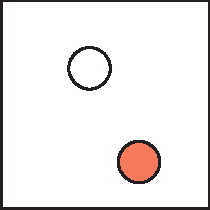
\includegraphics[width=1.5in]{images/samplefigure}
  \caption{Sample illustration.}
  \label{FIG:SAMPLE}
\end{figure}

\section*{Acknowledgements}

To my mum, my dad, and the dog. 

\bibliographystyle{acmsiggraph}
\bibliography{template}
\end{document}
